% !TEX root = report.tex

\subsection{Further Analysis}
\label{app:further_analysis}

\subsubsection{Impact of the dimensionality reduction}
\label{app:dim_reduction}
Working with large sized vectors of features can be very memory and time demanding, especially when training a complex classifier, maybe with a large number of parameters. For this reason one usually implement, before passing the data to the algorithm, a dimensionality reduction step, that in this case is a \textit{Principal Component Analysis}, with the purpose of reducing the dimension of each input vector, while keeping the "information" provided by it as untouched as possible. But how much this step will influence the performances of the classifiers? Let's first give a look at figure \ref{fig:cev}, that allows to determine the number of principal components to keep without losing too much of that "information". Basically, during the PCA, you are projecting your data into a smaller dimensional vector space, and each principal component corresponds to an eigenvalue of the covariance matrix of the dataset: reducing the size of the problem means keeping only the first $K$ eigenvalues, i.e. the ones with the higher variance. In the plot it is represented the \textit{cumulative explained variance} as a function of the number of components kept: the closer to 1 is the value, the more will be the information represented.
\begin{figure}[!h]
	\centering
	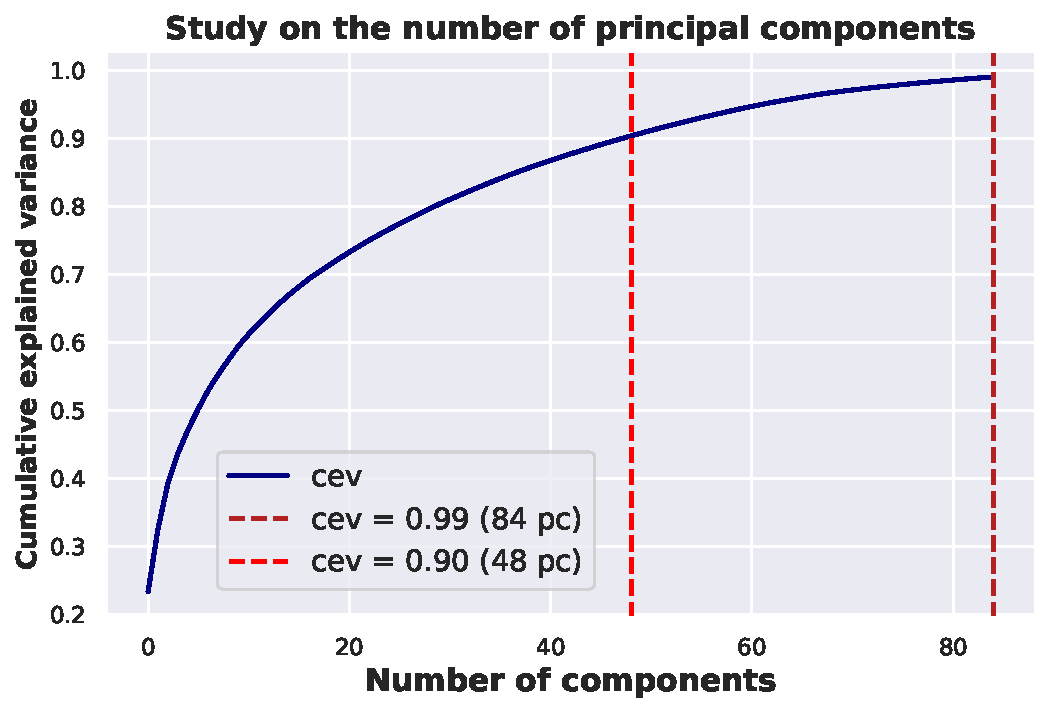
\includegraphics[width=0.4\textwidth]{pictures/cev.pdf}
	\caption{Cumulative explained variance ratio of the Principal Component Analysis applied to the features dataset.}
	\label{fig:cev}
\end{figure}
Looking at the line, one clearly see that, potentially, the 90\% of the information stored in the features can be reduced to just 48 values! The analysis presented in section \ref{sec:results} have been computed keeping, by default, the 99\% of the explained variance, i.e. 84 principal components. And the results are still quite nice. What would happen, instead, further reducing the number of eigenvalues to keep?
\begin{figure}[!h]
	\centering
	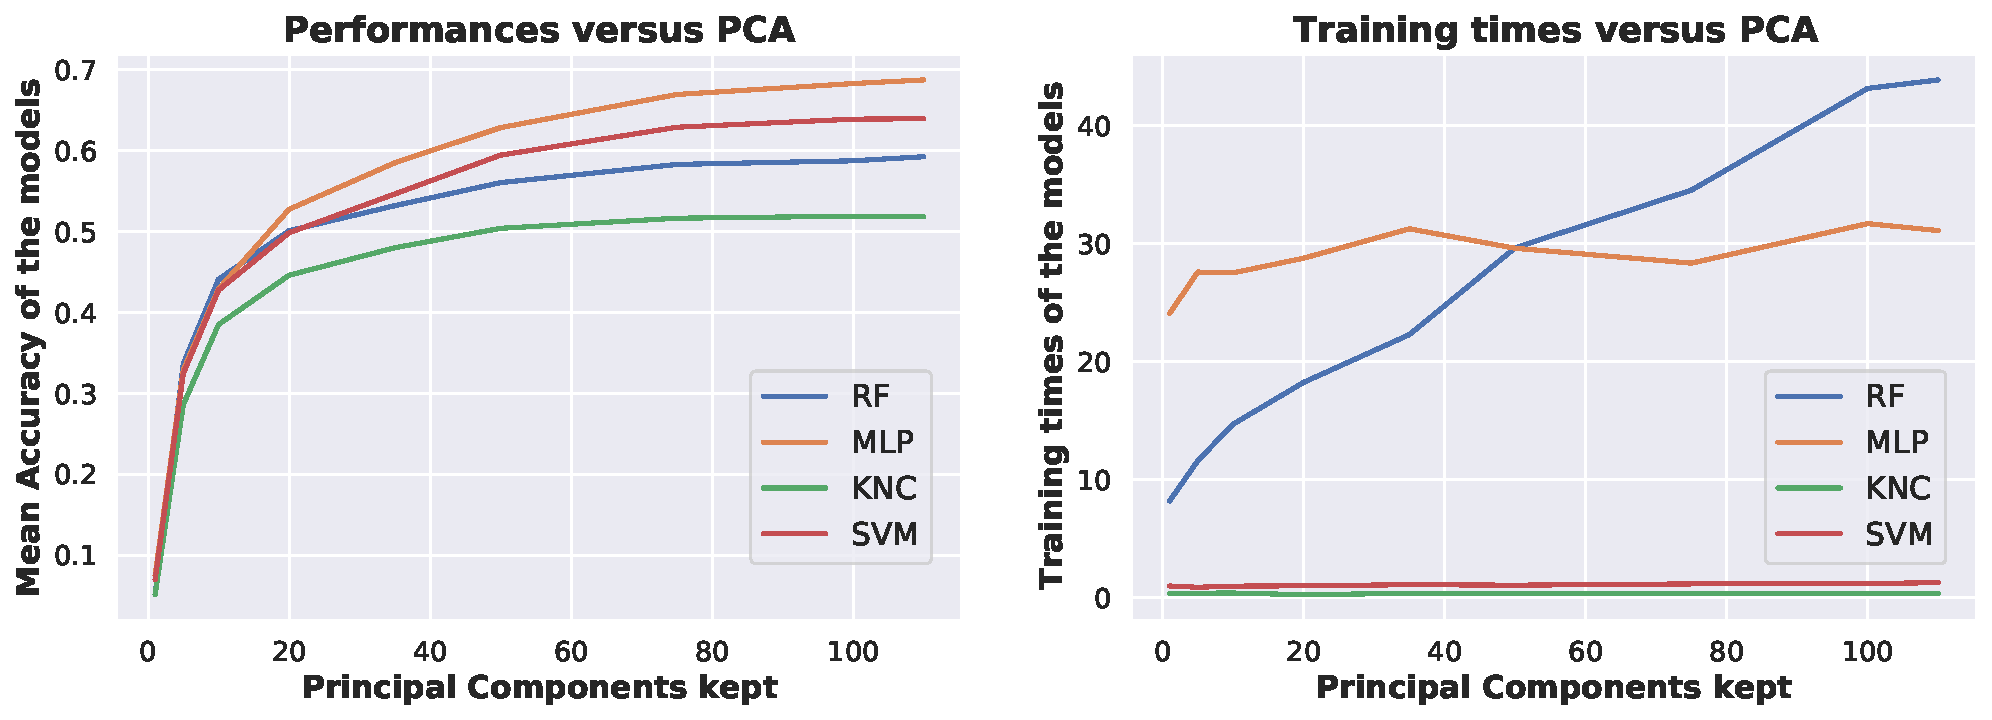
\includegraphics[width=0.5\textwidth]{pictures/pca_analysis.pdf}
	\caption{Comparison of mean accuracy reached and training times of the models for different numbers of principal components kept.}
	\label{fig:pca_analysis}
\end{figure}
The results shown in figure \ref{fig:pca_analysis} looks like exactly what we expected:
\begin{itemize}
	\itemsep0em
	\item in the left plot there are the mean accuracies obtained for the models trained: already after 40/50 principal components the lines start becoming flat, meaning that no significant further improvements are possible. And this is coherent with the explained variance ratio presented before (figure \ref{fig:cev}). Recalling section \ref{sec:features_extraction}, the vectors aimed to provide an high-level representation of the clips were created using an high number of features: probably so many (55) different quantities were unnecessary, and only half of them were sufficient. However, properly tuning the number of principal components, the problem vanishes.
	\item the right plot, instead, shows the computational times: the bigger are the input vectors, the larger will be the time necessary to make the classifier learn from them. With just 2000 clips the absolute difference is not so relevant, but the scaling behaviors of the lines, instead, are evident.
\end{itemize}


\subsubsection{Importance of the statistical estimators for the features distributions}
\label{app:stat_estimators}
In section \ref{sec:features_extraction} it has been explained that features distributions across frames were "summarized" using also their standard deviation, together with their mean, in order to properly represent also their irregularity and asymmetry. In figure \ref{fig:stat_estimators} it is shown the effective improvement, in term of accuracy, achieved training the four machine learning classifiers using just the mean or both the mean and the standard deviation.
\begin{figure}[!h]
	\centering
	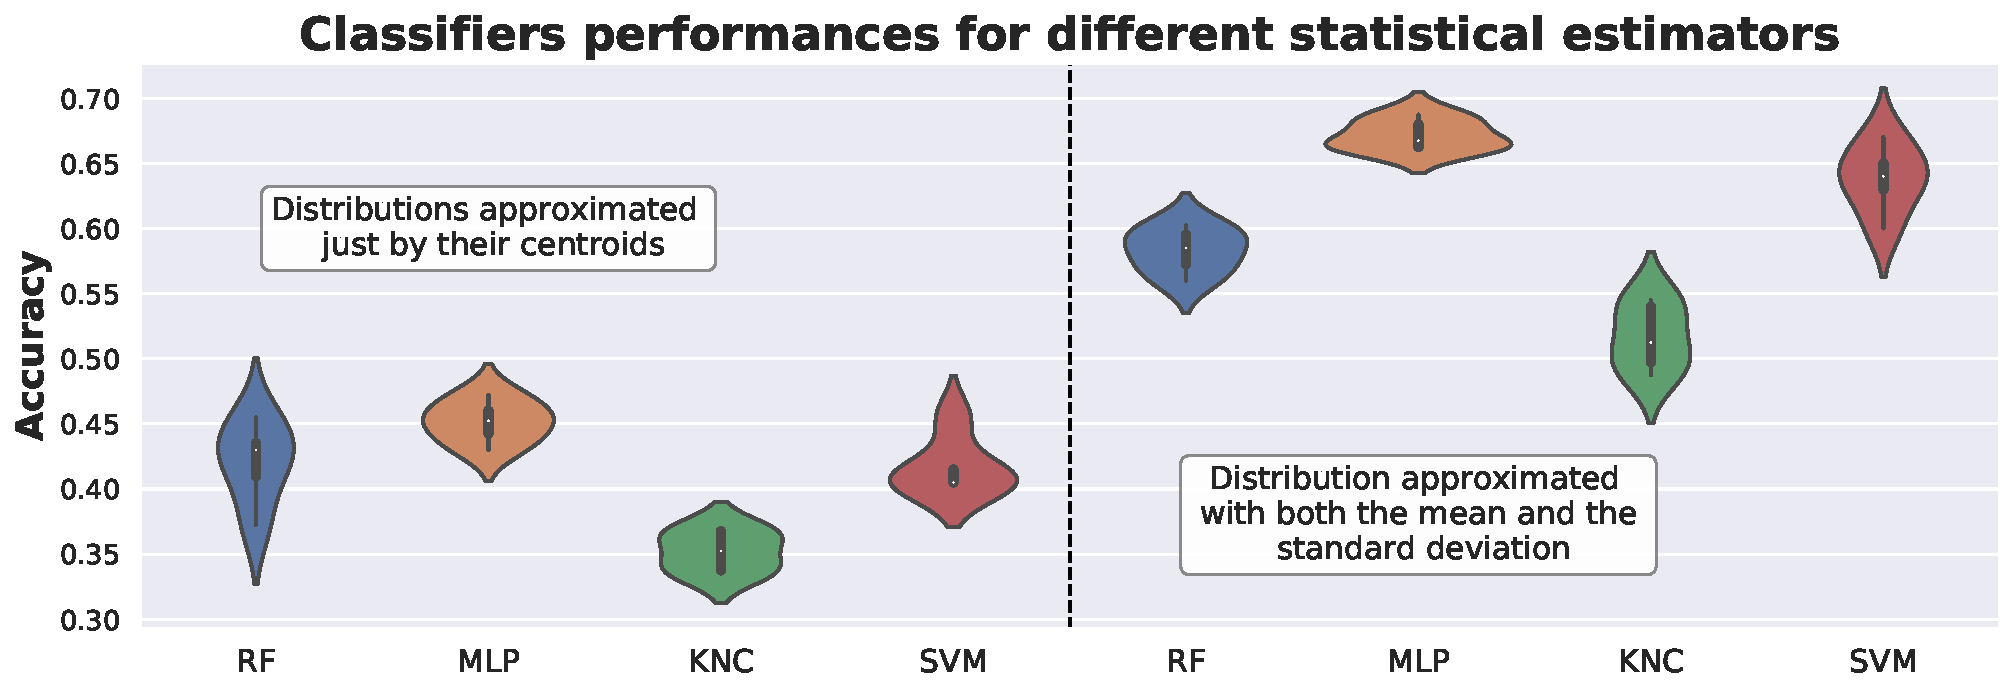
\includegraphics[width=0.47\textwidth]{pictures/stat_estimators.pdf}
	\caption{Comparison of the accuracy reached by the classifiers with one or two statistical estimators representing features distributions.}
	\label{fig:stat_estimators}
\end{figure}
The improvement is obvious: using both the mean and the standard deviation as statistics estimators provides almost a $+20\%$ to the accuracy obtained with all the models used. As expected, in fact, the distributions are, in general, quite asymmetric and non-gaussian, and taking just the average is probably an excess of reductionism.


\subsubsection{Importance of the silence removal step}
\label{app:importance_windowing}
The last step of the preprocessing phase explained in section \ref{sec:windowing} was the silence removal, i.e. the identification of fixed-size windows of zero energy, and their remotion from the successive calculations. In figure 	\ref{fig:silence_removal} are shown the differences, in term of accuracy, obtained with and without this windowing procedure.
\begin{figure}[!t]
	\centering
	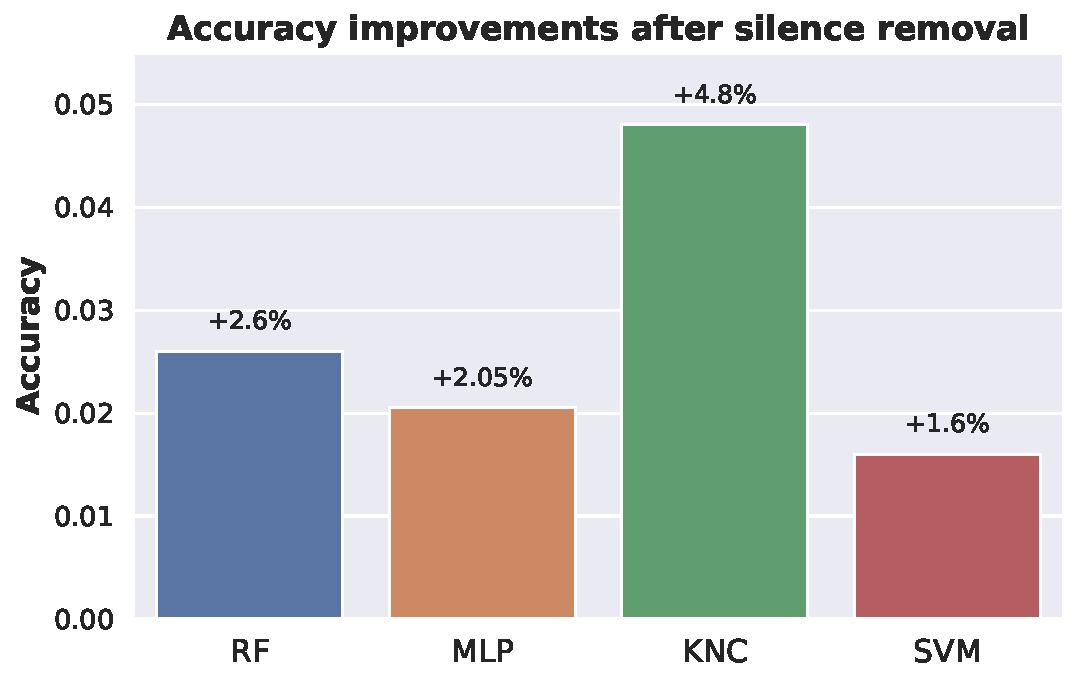
\includegraphics[width=0.47\textwidth]{pictures/silence_removal.pdf}
	\caption{Effective improvements in accuracy reached training the models with and without the silence removal phase.}
	\label{fig:silence_removal}
\end{figure}
And this is not even bad: getting a $+1\%/+5\%$ improvement in accuracy is nice, at the expenses of a small further preprocessing step.

